\begin{figure}[h!]
    \centering
    \caption{Estimated shares pocketed by landlords under a counterfactual increase 
             in the federal minimum wage to \$9, urban ZIP codes}
    \label{fig:cf_hist_rents_wages_shares}

    \begin{subfigure}{0.65\textwidth}
        \caption*{Share of additional income pocketed by landlords}
        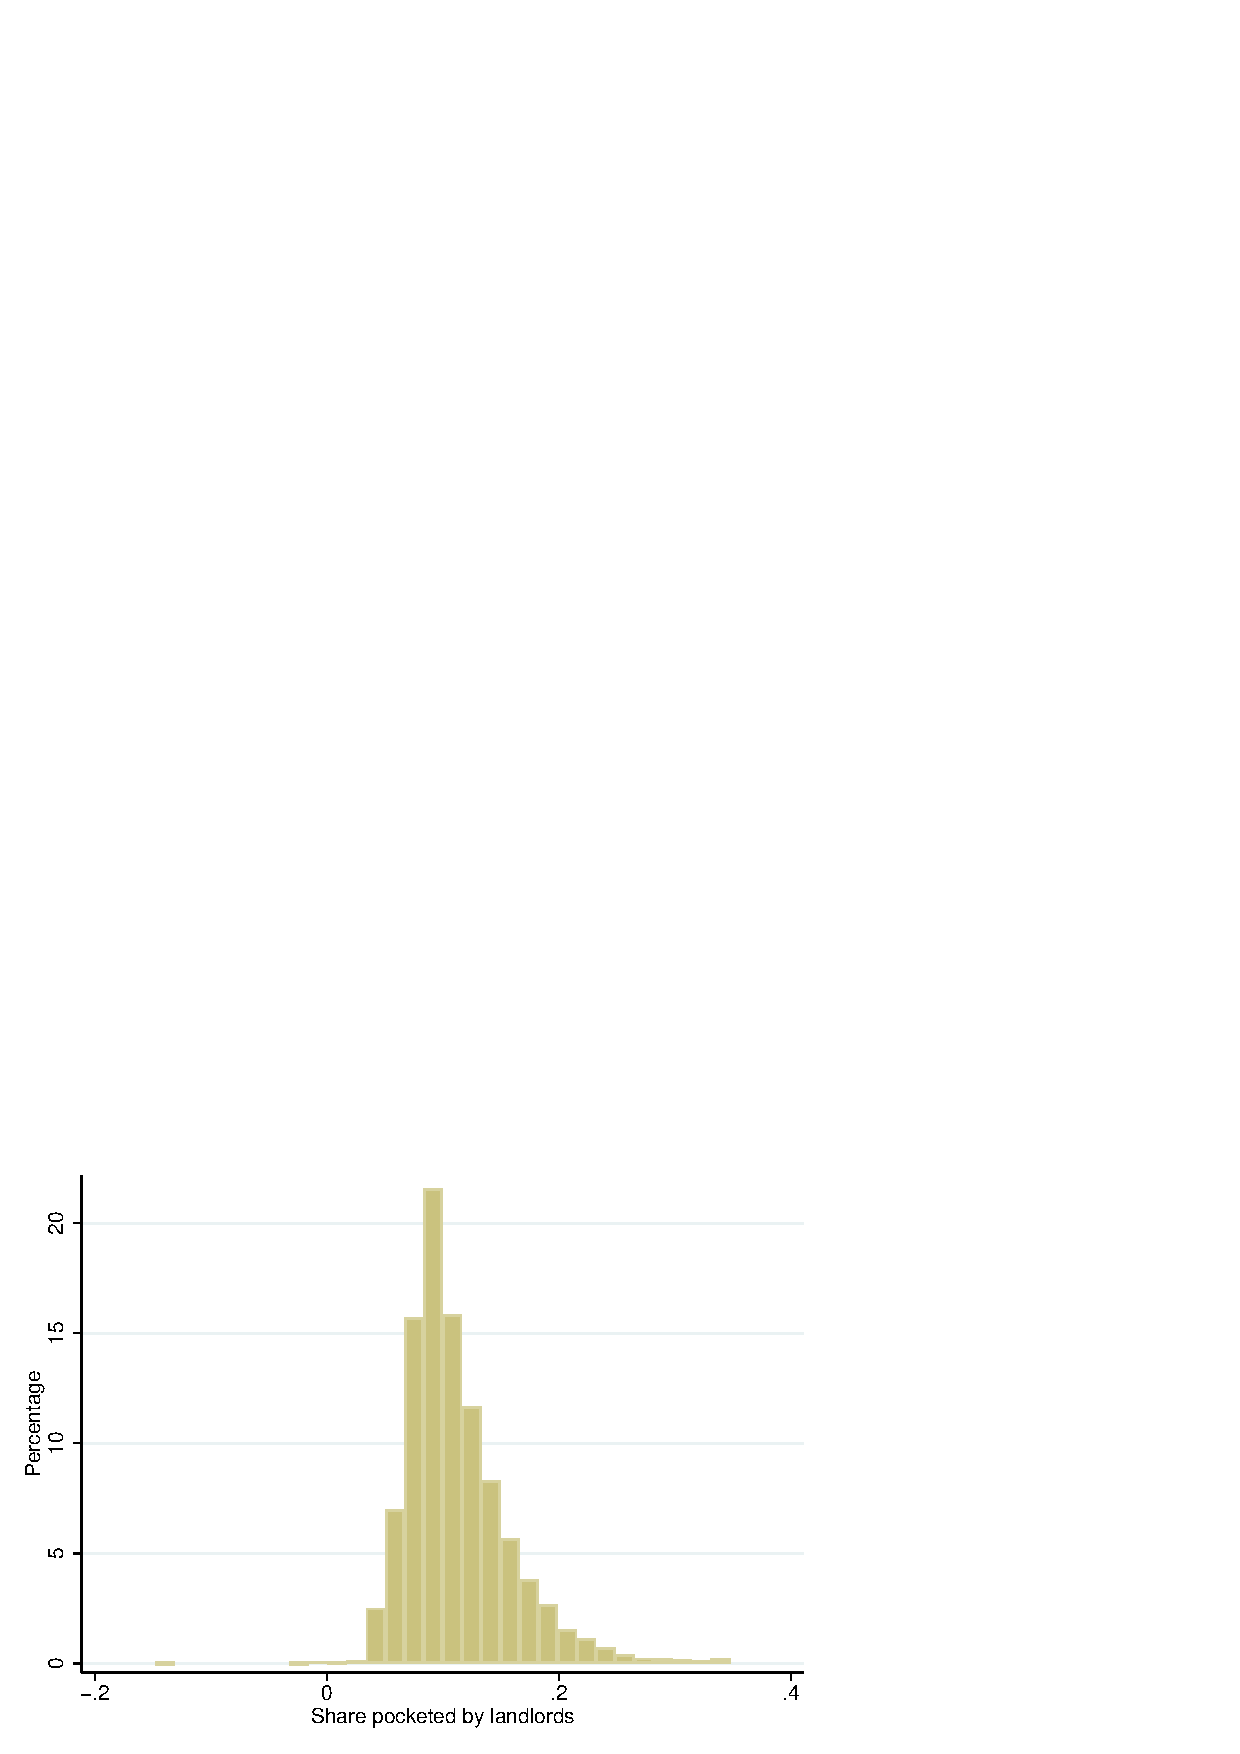
\includegraphics[width = 1\textwidth]{counterfactuals/output/hist_rho_with_imputed_fed_9usd}
    \end{subfigure}\\
    \begin{subfigure}{0.5\textwidth}
        \caption*{Change in log rents}
        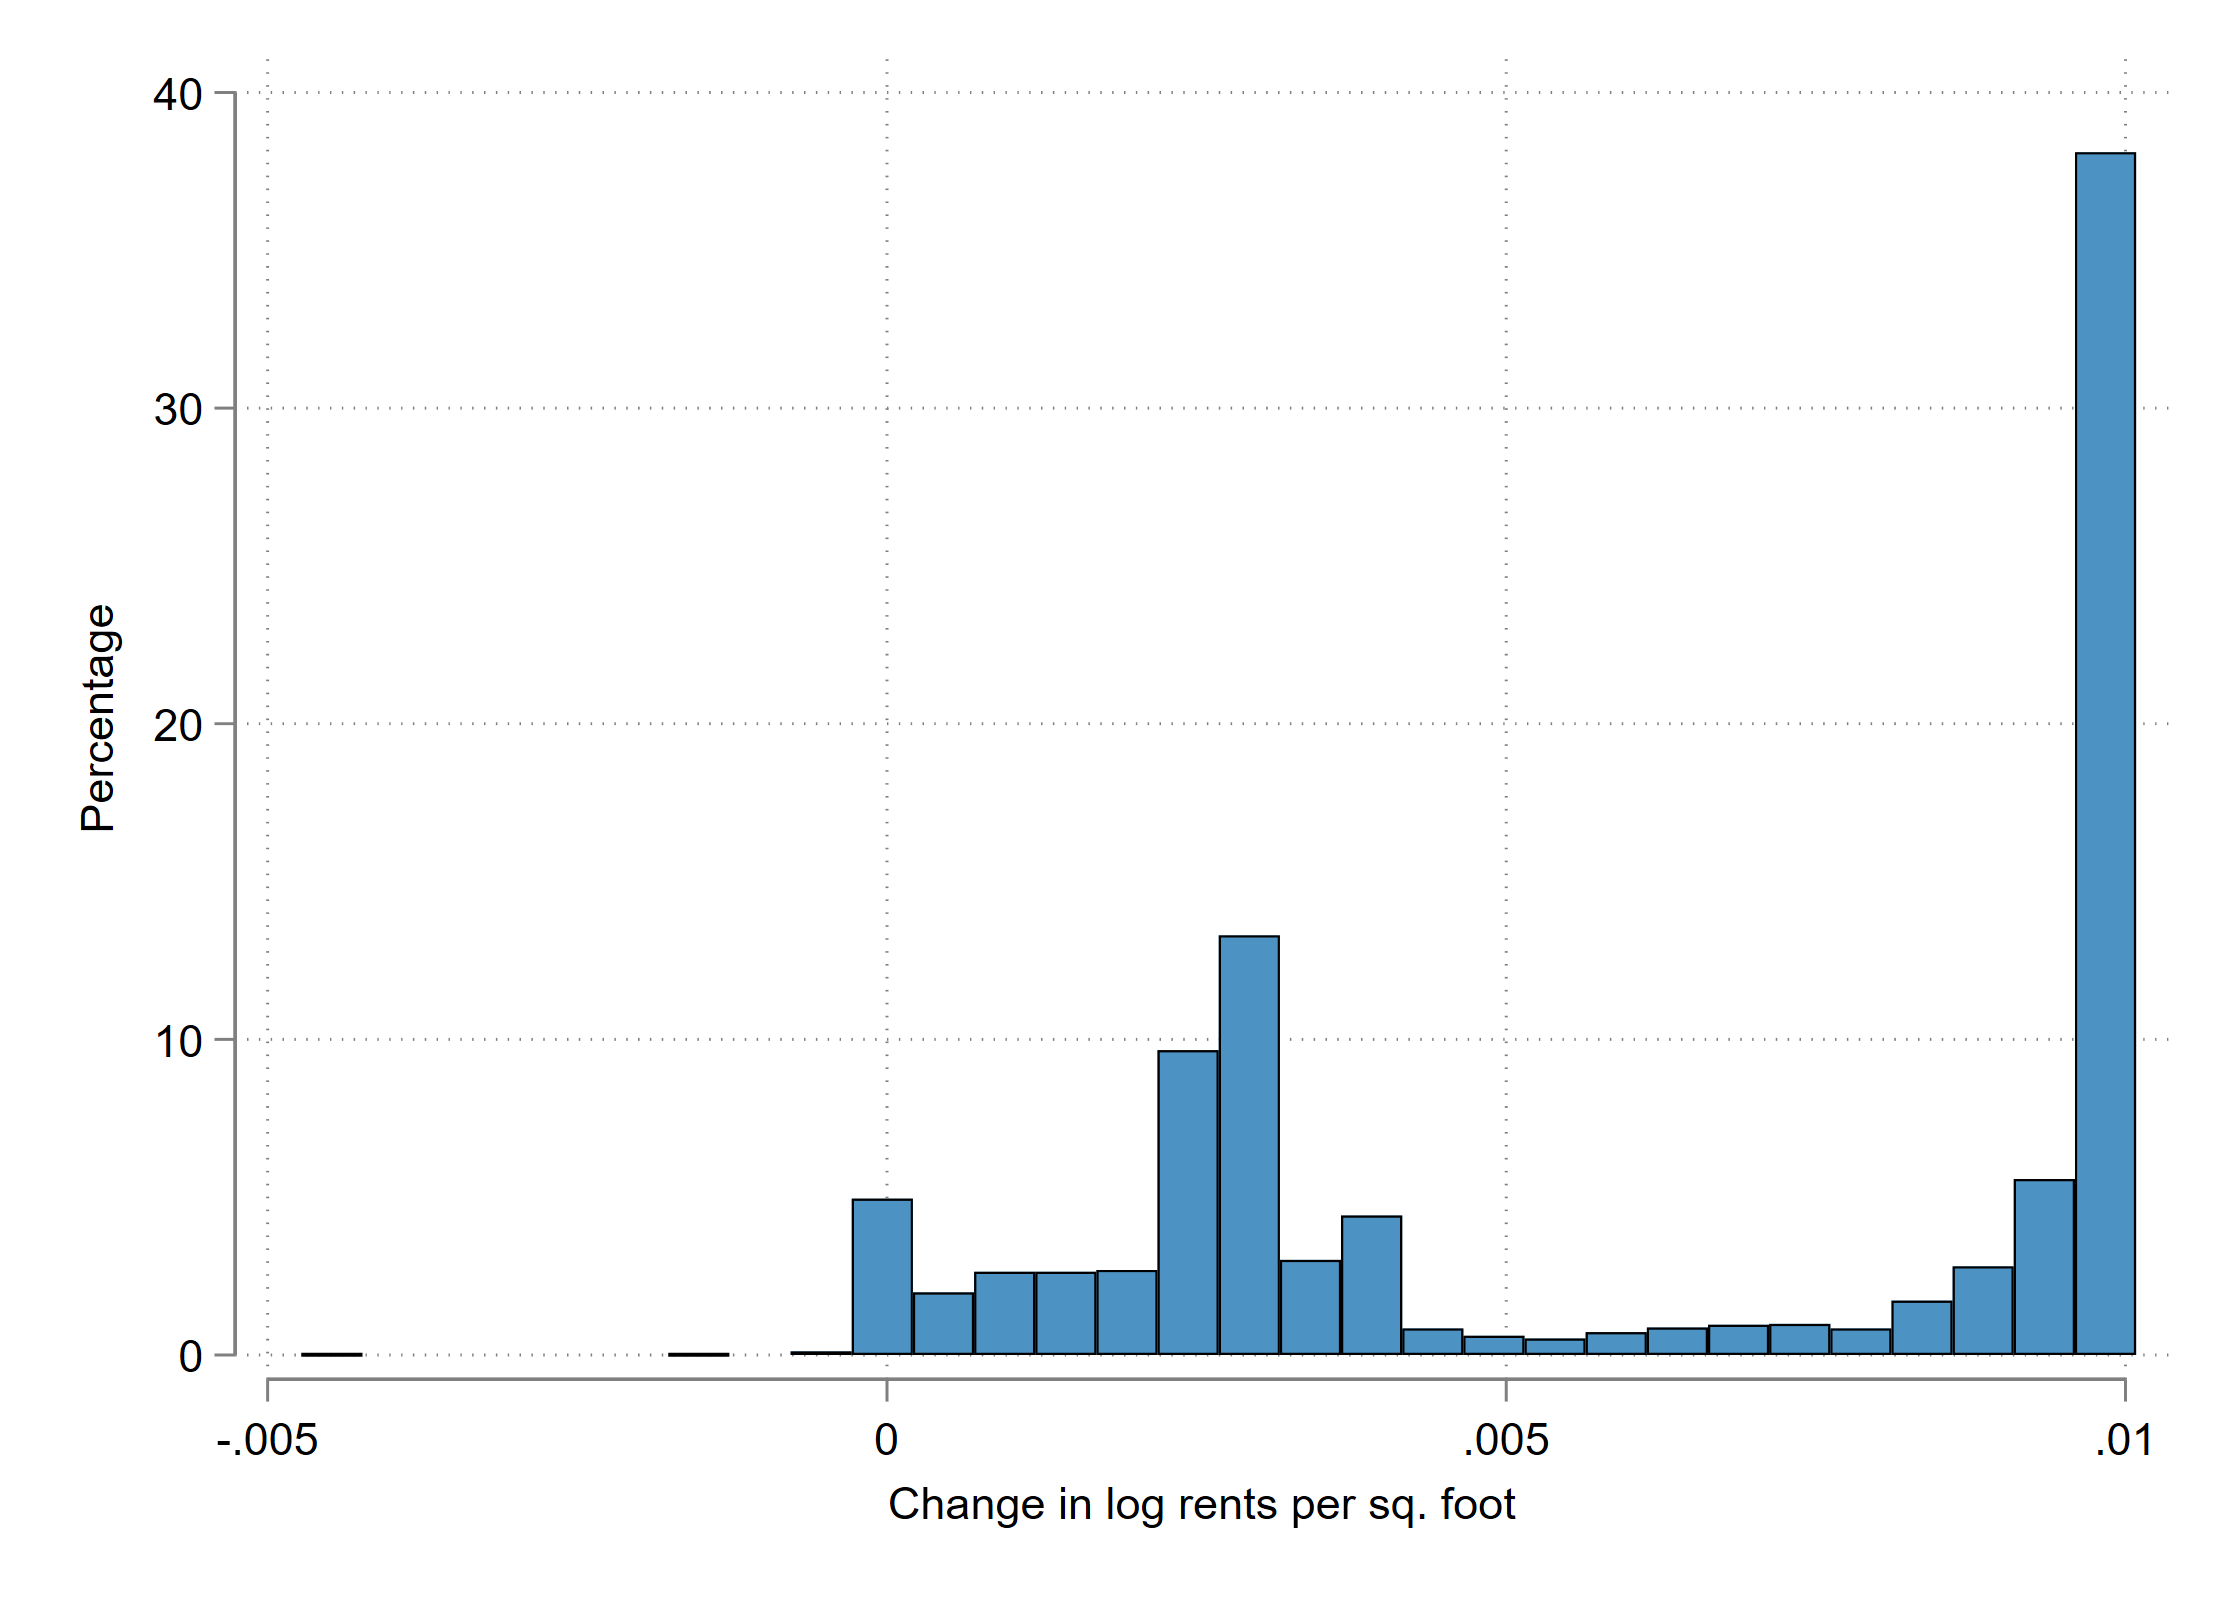
\includegraphics[width = .95\textwidth]{counterfactuals/output/hist_change_ln_rents_fed_9usd}
    \end{subfigure}%
    \begin{subfigure}{0.5\textwidth}
        \caption*{Change in log total wages}
        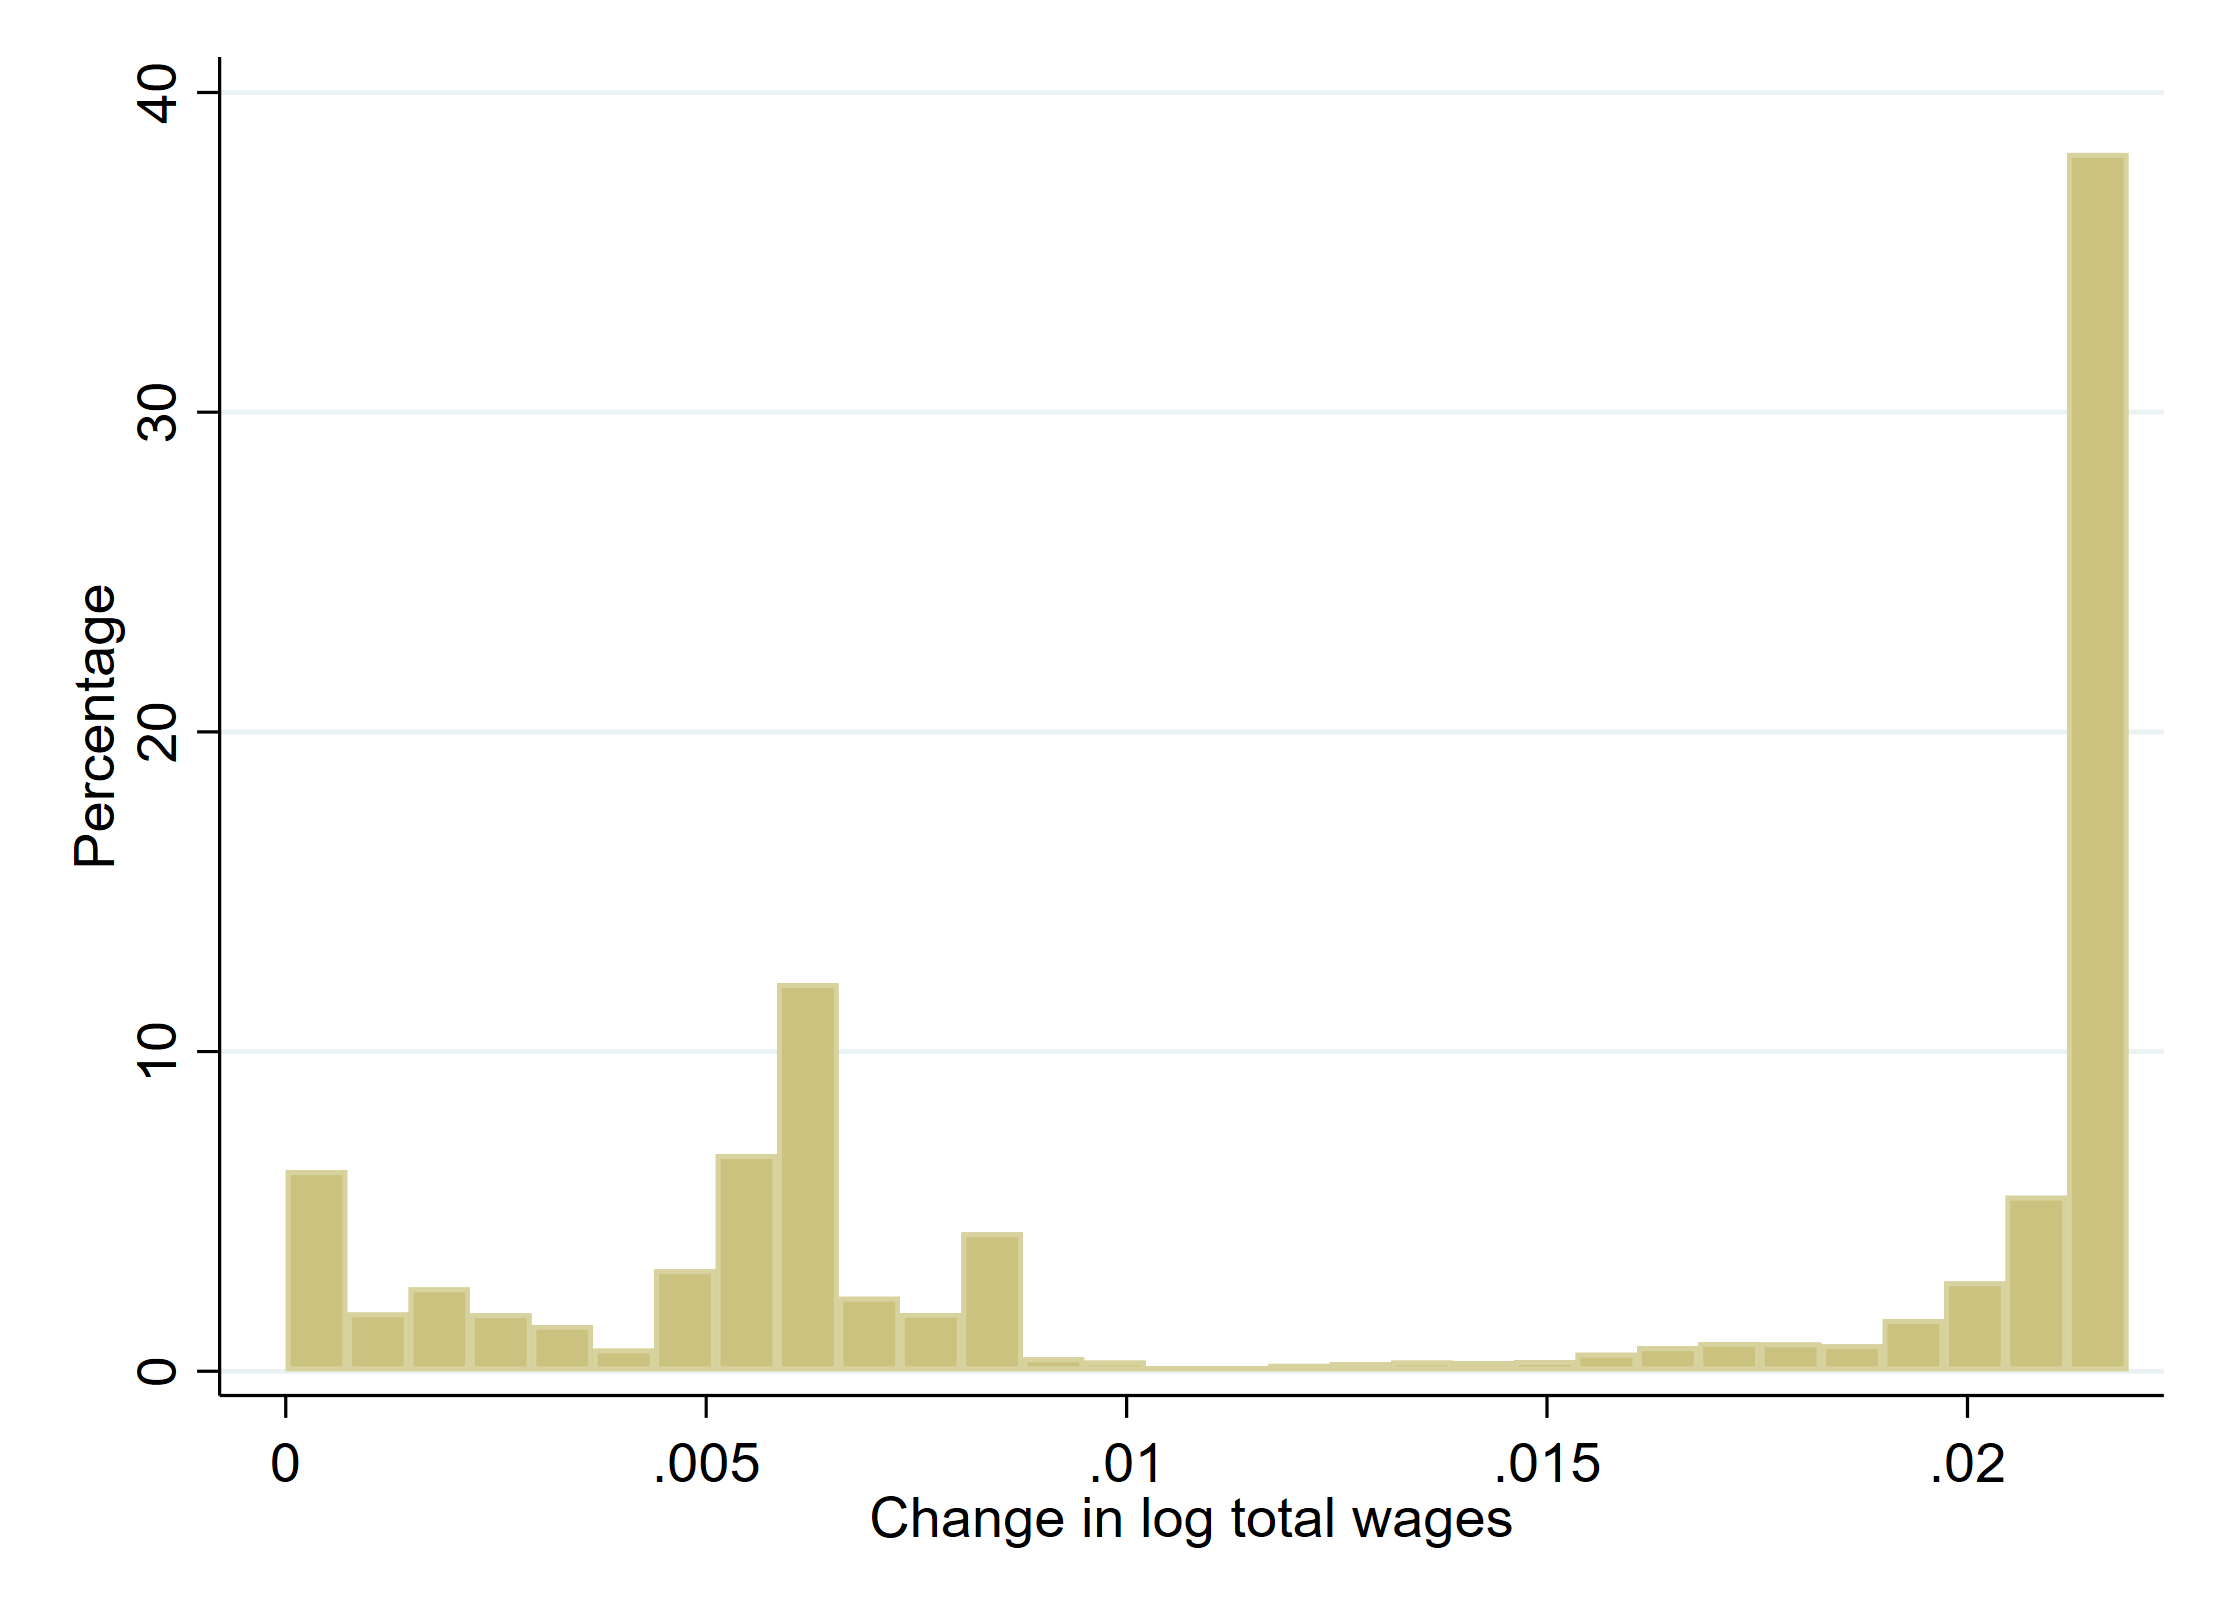
\includegraphics[width = .95\textwidth]{counterfactuals/output/hist_change_ln_wagebill_fed_9usd}
    \end{subfigure}

    \begin{minipage}{.95\textwidth} \footnotesize
        \vspace{3mm}
        Notes:
        Data are from the MW panel described in section \ref{sec:data_mw_panel} 
        and from LODES.
        The top figure shows the distribution of the estimated ZIP-code specific
        shares of the additional income pocketed by landlords (``share pocketed''), 
        the bottom left figure shows estimated changes in log rents, and 
        the bottom right figure shows estimated changes in log total wages.
        The computations are based on a counterfactual increase to \$9 in the 
        federal MW in January 2020, holding constant other MW policies in their 
        December 2019 levels.
        The unit of observation is the urban ZIP code, where we define a ZIP code 
        as urban if it belongs to a CBSA with at least 80\% of its population 
        classified as urban by the 2010 Census.
        The share pocketed is defined as the ratio between the percent increase 
        in rents and the percent increase in total wages multiplied by the share 
        of housing expenditure in the ZIP code.
        To estimate it we follow the procedure described in Section 
        \ref{sec:counterfactual}, assuming the following parameter values: 
        $\beta = 0.0546$, $\gamma = -0.0207$, $\varepsilon = 0.1083$, and 
        $s = 0.35$.
        We exclude 5 ZIP codes for which the estimated landlord share was 
        below $-1$.
    \end{minipage}
\end{figure}
